%-----------------------------------------------------------------------------------------------------------------------------------------------%
%	The MIT License (MIT)
%
%	Copyright (c) 2015 Jan Küster
%
%	Permission is hereby granted, free of charge, to any person obtaining a copy
%	of this software and associated documentation files (the "Software"), to deal
%	in the Software without restriction, including without limitation the rights
%	to use, copy, modify, merge, publish, distribute, sublicense, and/or sell
%	copies of the Software, and to permit persons to whom the Software is
%	furnished to do so, subject to the following conditions:
%	
%	THE SOFTWARE IS PROVIDED "AS IS", WITHOUT WARRANTY OF ANY KIND, EXPRESS OR
%	IMPLIED, INCLUDING BUT NOT LIMITED TO THE WARRANTIES OF MERCHANTABILITY,
%	FITNESS FOR A PARTICULAR PURPOSE AND NONINFRINGEMENT. IN NO EVENT SHALL THE
%	AUTHORS OR COPYRIGHT HOLDERS BE LIABLE FOR ANY CLAIM, DAMAGES OR OTHER
%	LIABILITY, WHETHER IN AN ACTION OF CONTRACT, TORT OR OTHERWISE, ARISING FROM,
%	OUT OF OR IN CONNECTION WITH THE SOFTWARE OR THE USE OR OTHER DEALINGS IN
%	THE SOFTWARE.
%	
%
%-----------------------------------------------------------------------------------------------------------------------------------------------%


%============================================================================%
%
%	DOCUMENT DEFINITION
%
%============================================================================%

%we use article class because we want to fully customize the page and dont use a cv template
\documentclass[10pt,A4]{article}	


%----------------------------------------------------------------------------------------
%	ENCODING
%----------------------------------------------------------------------------------------

%we use utf8 since we want to build from any machine
\usepackage[utf8]{inputenc}		

%----------------------------------------------------------------------------------------
%	LOGIC
%----------------------------------------------------------------------------------------

% provides \isempty test
\usepackage{xifthen}

%----------------------------------------------------------------------------------------
%	FONT
%----------------------------------------------------------------------------------------

% some tex-live fonts - choose your own

%\usepackage[defaultsans]{droidsans}
%\usepackage[default]{comfortaa}
%\usepackage{cmbright}
\usepackage[default]{raleway}
%\usepackage{fetamont}
%\usepackage[default]{gillius}
%\usepackage[light,math]{iwona}
%\usepackage[thin]{roboto} 

% set font default
\renewcommand*\familydefault{\sfdefault} 	
\usepackage[T1]{fontenc}

% more font size definitions
\usepackage{moresize}		


%----------------------------------------------------------------------------------------
%	PAGE LAYOUT  DEFINITIONS
%----------------------------------------------------------------------------------------

%debug page outer frames
%\usepackage{showframe}			

%add support for hyperlinks with href
\usepackage{hyperref}

%define page styles using geometry
\usepackage[a4paper]{geometry}		

% for example, change the margins to 2 inches all round
\geometry{top=.5cm, bottom=-.6cm, left=-0.1cm, right=0cm} 	

%use customized header
\usepackage{fancyhdr}				
\pagestyle{fancy}

%less space between header and content
\setlength{\headheight}{-5pt}		


%customize entries left, center and right
\lhead{}
\chead{}
\rhead{}

\newcommand{\padding}{1cm}
\newcommand{\innerwidth}{\linewidth-\padding-\padding}

%indentation is zero
\setlength{\parindent}{0mm}

%----------------------------------------------------------------------------------------
%	TABLE /ARRAY DEFINITIONS
%---------------------------------------------------------------------------------------- 

%for layouting tables
\usepackage{multicol}			
\usepackage{multirow}

%extended aligning of tabular cells
\usepackage{array}

\newcolumntype{x}[1]{%
>{\raggedleft\hspace{0pt}}p{#1}}%


%----------------------------------------------------------------------------------------
%	GRAPHICS DEFINITIONS
%---------------------------------------------------------------------------------------- 

%for header image
\usepackage{graphicx}

%for floating figures
\usepackage{wrapfig}
\usepackage{float}
%\floatstyle{boxed} 
%\restylefloat{figure}

%for drawing graphics		
\usepackage{tikz}				
\usetikzlibrary{shapes, backgrounds,mindmap, trees}


%----------------------------------------------------------------------------------------
%	Color DEFINITIONS
%---------------------------------------------------------------------------------------- 
\usepackage{transparent}
\usepackage{color}

%accent color
\definecolor{sectcol}{RGB}{175,89,153}

%dark background color
\definecolor{bgcol}{RGB}{68,68,132}

%light background / accent color
\definecolor{softcol}{RGB}{231,171,180}

% light bg
\definecolor{light}{RGB}{169,171,210}

%============================================================================%
%
%
%	DEFINITIONS
%
%
%============================================================================%

%----------------------------------------------------------------------------------------
% 	HEADER
%----------------------------------------------------------------------------------------

% remove top header line
\renewcommand{\headrulewidth}{0pt} 

%remove botttom header line
\renewcommand{\footrulewidth}{0pt}	  	

%remove pagenum
\renewcommand{\thepage}{}	

%remove section num		
\renewcommand{\thesection}{}			

%----------------------------------------------------------------------------------------
% 	ARROW GRAPHICS in Tikz
%----------------------------------------------------------------------------------------

% a six pointed arrow poiting to the left
\newcommand{\tzlarrow}{(0,0) -- (0.2,0) -- (0.3,0.2) -- (0.2,0.4) -- (0,0.4) -- (0.1,0.2) -- cycle;}	

% include the left arrow into a tikz picture
% param1: fill color
%
\newcommand{\larrow}[1]
{\begin{tikzpicture}[scale=0.58]
	 \filldraw[fill=#1!100,draw=#1!100!black]  \tzlarrow
 \end{tikzpicture}
}

% a six pointed arrow poiting to the right
\newcommand{\tzrarrow}{ (0,0.2) -- (0.1,0) -- (0.3,0) -- (0.2,0.2) -- (0.3,0.4) -- (0.1,0.4) -- cycle;}

% include the right arrow into a tikz picture
% param1: fill color
%
\newcommand{\rarrow}[1]
{\begin{tikzpicture}[scale=0.7]
	 \filldraw[fill=#1!100,draw=#1!100!black]  \tzrarrow
 \end{tikzpicture}
}



%----------------------------------------------------------------------------------------
%	custom sections
%----------------------------------------------------------------------------------------

% create a coloured box with arrow and title as cv section headline
% param 1: section title
%
\newcommand{\cvsection}[1]
{
\colorbox{sectcol}{\mystrut \makebox[1\linewidth][l]{
\larrow{bgcol} \hspace{-8pt} \larrow{bgcol} \hspace{-8pt} \larrow{bgcol} \textcolor{white}{\textbf{#1}}\hspace{4pt}
}}\\
}

%create a coloured arrow with title as cv meta section section
% param 1: meta section title
%
\newcommand{\metasection}[2]
{
\begin{tabular*}{1\textwidth}{p{2cm} p{11cm}}
\larrow{bgcol}	\normalsize{\textcolor{sectcol}{#1}}&#2\\[8pt]
\end{tabular*}
}

%----------------------------------------------------------------------------------------
%	 CV EVENT
%----------------------------------------------------------------------------------------

% creates a stretched box as cv entry headline followed by two paragraphs about 
% the work you did
% param 1:	event time i.e. 2014 or 2011-2014 etc.
% param 2:	event name (what did you do?)
% param 3:	institution (where did you work / study)
% param 4:	what was your position
% param 5:	some words about your contributions
%
\newcommand{\cvevent}[5]
{
\vspace{8pt}
	\begin{tabular*}{0.6\linewidth}{ p{12cm} x{3cm}}
\textbf{#2} \textcolor{bgcol}{(#3)}&\textcolor{bgcol}{#1}\\[4pt]
	\end{tabular*}
\vspace{-12pt}
\textcolor{softcol}{\hrule}
\vspace{6pt}
	\begin{tabular*}{1\textwidth}{l}
		 \larrow{sectcol}  #4\\[4.5pt]
		 \larrow{sectcol}  #5\\[6pt]
	\end{tabular*}
\vspace{-4pt}
}

% creates a stretched box as 
\newcommand{\cveventmeta}[2]
{
	\mbox{\mystrut \hspace{87pt}\textit{#1}}\\
	#2
}

%----------------------------------------------------------------------------------------
% CUSTOM STRUT FOR EMPTY BOXES
%----------------------------------------- -----------------------------------------------
\newcommand{\mystrut}{\rule[-.3\baselineskip]{0pt}{\baselineskip}}

%----------------------------------------------------------------------------------------
% CUSTOM LOREM IPSUM
%----------------------------------------------------------------------------------------
\newcommand{\lorem}
{Lorem ipsum dolor sit amet, consectetur adipiscing elit. Donec a diam lectus.}



%============================================================================%
%
%
%
%	DOCUMENT CONTENT
%
%
%
%============================================================================%
\begin{document}

%use our custom fancy header definitions
\pagestyle{fancy}	

%----------------------------------------------------------------------------------------
% HEADLINE / BASIC INFORMATION
%----------------------------------------------------------------------------------------
\fcolorbox{bgcol}{bgcol}{
\begin{minipage}[c][0.085\textheight][t]{\linewidth}
\begin{center}
	\vspace{14pt}
	\textcolor{light}{\small{Electrónica, Programación, Ciberseguridad $\cdot$ Argentina $\cdot$  \href{mailto:randazzoignacio@gmail.com}{randazzoignacio@gmail.com} }}\\
	\HUGE{\textcolor{white}{\textsc{Ignacio Randazzo}} } \textcolor{sectcol}{\rule[-1mm]{1mm}{0.9cm}} \HUGE{\textcolor{white}{\textsc{CV}} }
\end{center}
\end{minipage}}\\[-4pt]
%----------------------------------------------------------------------------------------
% SUMMARY
%----------------------------------------------------------------------------------------
\fcolorbox{sectcol}{sectcol}{
\begin{minipage}[c][0.03\textheight][t]{\linewidth}
\vspace{-3pt}
\begin{center}
\parbox[b]{0.75\linewidth}{
	\begin{center}
	\larrow{bgcol}\larrow{bgcol} \textcolor{white}{Pueden encontrar la última versión de este CV en \href{https://randazzo.ar/cv}{randazzo.ar/cv} } \rarrow{bgcol}\rarrow{bgcol}
	\end{center}
}
\end{center}
\end{minipage}}\\[-4pt]
%----------------------------------------------------------------------------------------
% META
%----------------------------------------------------------------------------------------
\fcolorbox{white}{white}{
\begin{minipage}[c][0.16\textheight][t]{\linewidth}
\vspace{8pt}
\begin{center}
\parbox[c]{\innerwidth}{
  \begin{tikzpicture}
    \clip (0,0) circle(0.1\linewidth);
    \node at (0,0) {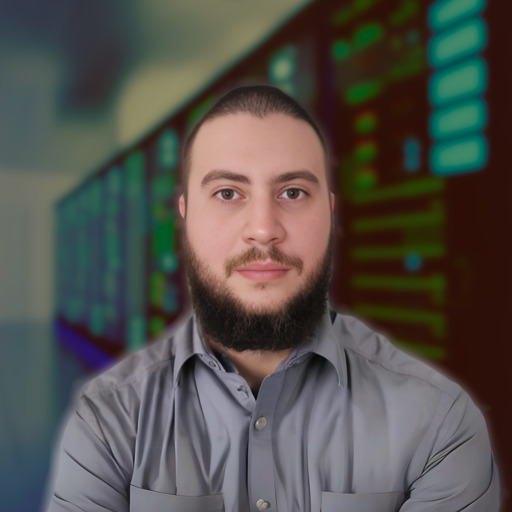
\includegraphics[width=0.2\linewidth]{profile.jpg}};
  \end{tikzpicture}
	\hspace{8pt}
	\parbox[b]{5cm}{
	\metasection{Estado:}{Busqueda laboral activa. Trabajando en mi tésis de grado.}
	\metasection{Campos:}{Electrónica, Programación, Ciberseguridad}
	\metasection{Langs:}{C, C++, Bash, Python, Ruby, Verilog, VHDL}
	\metasection{Tools:}{Linux, Git, Ansible, Nginx, LaTeX, KiCAD}
	\metasection{Proyectos:}{CTF's, Game Jams, Proyectos Personales}
	}
}
\end{center}
\end{minipage}}\\[-4pt]
%----------------------------------------------------------------------------------------
% EXPERIENCE
%----------------------------------------------------------------------------------------
\fcolorbox{light}{light}{
\begin{minipage}[c][0.36\textheight][t]{\linewidth}
\vspace{4pt}
\hspace{26pt}
\parbox[c]{0.75\linewidth}{
%
\cvevent{2021 - 2023}{Ingeniero RTL ASIC}{Marvell Technology}{Diseño digital coherente de alta velocidad para ASIC de fibra óptica.}{System-Verilog para diseño y C++ para simulación.}

%\textcolor{softcol}{\hrule}

%
\cvevent{2020 - 2021}{Asistente de investigación}{Fundación Fulgor}{Diseño, implementación y verificación en FPGA.}{Canal de comuncaciones reconfigurable en tiempo real para chips de DPS para emulación.}


%\textcolor{softcol}{\hrule}

%
\cvevent{2017 - 2021}{Linux SysAdmin}{CIII UTN FRC}{Principal tarea instalación, administración y soporte del servidor Linux del centro de investigación.}{Proyectos de tiempo parcial incluyendo Machine Learning y análisis de imágenes con OpenCV.}

%\textcolor{softcol}{\hrule}

%
\cvevent{2019}{Desarrolo en Linux, y auditoría de seguridad}{Consultor para DIUCCO}{Instalación mantenimiento y segurización de Linux para máquina de voto electrónico.}{Auditoría de seguridad, con sus respectivos reportes, propuestas de mejoras, e implementación.}

%\textcolor{softcol}{\hrule}


%
\cvevent{2018}{Desarrollo de Linux embebido}{Biotero del Hospital de Cordoba}{Instalación y mantenimiento de Linux embebido para balanza inteligente.}{Desarrollo en C para interfacear Linux con hardware específico.}

}
\hspace{18pt}
\textcolor{sectcol}{\rule[-3.2cm]{2pt}{7cm}}
\hspace{12pt}
\rotatebox[origin=c]{270}{\HUGE \textsc{Experiencia}}
\end{minipage}}\\[-4pt]
%----------------------------------------------------------------------------------------
% SUMMARY
%----------------------------------------------------------------------------------------
\fcolorbox{bgcol}{bgcol}{
\begin{minipage}[c][0.03\textheight][t]{\linewidth}
\vspace{-3pt}
\begin{center}
\parbox[b]{0.75\linewidth}{
	\begin{center}
	\textcolor{sectcol}{\textbf{\textit{"... True rebels fight against all odds, true rebels never give up, yet they cannot triumph alone ..."}}}
	\end{center}
}
\end{center}
\end{minipage}}\\[-4pt]
%----------------------------------------------------------------------------------------
% EDUCATION
%----------------------------------------------------------------------------------------
\fcolorbox{white}{white}{
\begin{minipage}[c][0.2875\textheight][t]{\linewidth}
\vspace{1pt}
\hspace{26pt}
\parbox[c]{0.75\linewidth}{
%\cvsection{Education}

\cvevent{2015 - 2025}{Ingeniería Electrónica}{Universidad Tecnológica Nacional}{Fecha estimada de presentación de tésis y graduación: Primer semestre 2025}{Promedio: 8/10.}

%\textcolor{softcol}{\hrule}

%
\cvevent{2024}{Google Cybersecurity Certificate}{Google}{Credencial: \href{https://www.credly.com/badges/8a242168-417a-4b6a-be9c-2b187e74cdda/public_url}{Google Cybersecurity Badge}}{Aspectos legales y regulatorios de ciberseguridad en detalle, no tanto así aspectos prácticos.}

%\textcolor{softcol}{\hrule}

%
\cvevent{2024}{Junior Cybersecurity Analyst}{Cisco}{Credencial: \href{https://www.credly.com/badges/17851325-7634-4f93-b3e3-934d3620d040/public_url}{Junior Cybersecurity Analyst Badge}}{Conceptos básicos de ciberseguridad, muchos conceptos cubiertos pero no tanta profundidad.}

%\textcolor{softcol}{\hrule}

%
\cvevent{2025}{Security+}{CISA}{Tanto aspectos prácticos como conceptos legales y regulatorios cubiertos en detalle.}{Curso ya completado, pero todavía resta por rendir el exámen de certificación.}

}
\hspace{18pt}
\textcolor{sectcol}{\rule[-3.2cm]{2pt}{7cm}}
\hspace{12pt}
\rotatebox[origin=c]{270}{\HUGE \textsc{Educación}}
\end{minipage}}\\[-4pt]
%---------------------------------------------------------------------------------------
%	QR CODE (optional)
%----------------------------------------------------------------------------------------
%\vspace{-136pt}
%\hspace{0.75\linewidth}
%\includegraphics[width=103pt]{qrcode}
%\normalsize
%\vspace{88pt}



%-------------------------------------------------------------------------------------------------
% FOOTER
%--------------------------------------------------------------------------------------------------
\fcolorbox{bgcol}{bgcol}{
\begin{minipage}[c][0.01\textheight][t]{\linewidth}
\vspace{-8pt}
\begin{center}
\parbox[b]{0.75\linewidth}{
	\begin{center}
	 \textcolor{white}{\href{https://randazzo.ar}{randazzo.ar}} \textcolor{white}{$\cdot$} \textcolor{white}{\href{https://www.linkedin.com/in/randazzo-ignacio/}{Linkedin}}
	\end{center}
}
\end{center}
\end{minipage}}
%============================================================================%
%
%
%
%	DOCUMENT END
%
%
%
%============================================================================%
\end{document}
